\documentclass{article}
\usepackage{cancel}
\usepackage{fullpage}
\usepackage{hyperref}
\usepackage{amsmath,amssymb,amsfonts,amsthm}
\usepackage{derivative}
\usepackage[parfill]{parskip}
\usepackage{graphicx}
\usepackage{cleveref}
%\usepackage{mathpazo}
%\usepackage[cmintegrals,cmbraces]{newtxmath}
\title{eSTA approach to Josephson Junction}
\date{}
\author{}
\usepackage{braket}
\DeclareMathOperator{\cas}{cas}
\newcommand{\trans}[1]{\ensuremath{{#1}^\intercal}}


\usepackage{color}

\setlength\parskip{2mm}
\begin{document}
\bibliographystyle{alpha}  
\maketitle
\section{The Bose Hubbard Hamiltonians}
In this section I will explain how to  move from the different definitions of Hamiltonians I encountered during this calculations. In particular I will try to connect the textbook example with the Hamiltonians used in \cite{FastGenerationJulia2012} and \cite{BoseEinsteinCJulia2010}.
Will do that later 
 
%%%%%%%%%%%%%%%%%%%%%%%%%
%Section where I summarize the STA to Josephson Junction
%%%%%%%%%%%%%%%%%%%%%%%%%
\section{Josephson Junction from the ground-up}
Here I will summarize the paper \cite{ABosonicJosepGati2007} where the Josephson Junction is derived.
We are considering  $ N $  particles in a double well potential, the form of which is
\begin{equation}
\label{eq:HamiltonianDoubleWell}
V_{dw} = \frac{1}{2} m \left(\omega^2_{x} x^2 + \omega^2_{y} y^2 + \omega^2_{z} z^2\right) + \frac{V_{0}}{2} \left(1 + \cos\frac{2\pi}{d_{sw}} x\right).
\end{equation}
Usually this problem is really hard to solve at involves many body particles etc. However the single particle spectrum of the double well is almost degenerate for the first two levels, while there is a wide gap between the second and third eigentates of the double well Hamiltonian.
This allows us to introduce the \textit{two mode approximation} in which only the first two eigentates are considered.
It has been shown how with this assumption the Hamiltonian of the system can be written as 
\begin{align}
\label{eq:HamiltonianDoubleWellIntegral}
& H = \hat{ H }_{0} + \hat{ H }_{int}\\
& \hat{H}_{0} = \int_{}^{}  \mathrm{d\mathbf{r}}\left(-\frac{\hbar^2}{2m} \hat{\Psi}^{\dag}\nabla^2\hat{ \Psi } + \hat{\Psi}^{\dag}V_{dw}\hat{ \Psi }\right)	,\\
& \hat{H}_{int} = \frac{g}{2}\int \mathrm{d\mathbf{r}} \hat{\Psi}^{\dag}\hat{\Psi}^{\dag}\hat{ \Psi }\hat{ \Psi }
\end{align}
with $ \hat{\Psi} $ field operator that (loosely speaking) creates / annihilates a particle in the position $ \mathbf{r} $ and $ g $ is the coupling constant.
Now we take into account only the mean-field ground and excited states (which I assume they are $\Phi_g = \ket{N,0}$ and  $\Phi_e = \ket{0,N})$ so we can rewrite the general wavefunction $\hat{ \Psi }$ as
\begin{equation}
\label{eq:GeneralState}
\hat{\Psi} = \hat{c}_{g}\Phi_g + \hat{c}_{e}\Phi_e
\end{equation}
with $\hat{c}_g^{\dagger} $ and $\hat{c}_e^{\dagger} $ the creation operator for the ground and excited states respectively.
A more convenient choice in this case is usually to choose the left and right operators
\begin{equation}
\label{eq:LeftRightOperators}
\hat{c}_l^{\dagger} = \frac{1}{\sqrt{2}  }\left( \hat{c}_g^{\dagger} + \hat{c}_e^{\dagger} \right)   \hspace{3em}\hat{c}_r^{\dagger} = \frac{1}{\sqrt{2}  }\left( \hat{c}_g^{\dagger} - \hat{c}_e^{\dagger} \right)  .
\end{equation}
With this choice, we can now rewrite $ \hat{\Psi} $ 
\begin{equation}
\label{eq:LeftRightPsi}
\hat{\Psi} = \frac{1}{\sqrt{2}}\left( \hat{c}_l(\Phi_g + \Phi_e) + \hat{c}_r(\Phi_g - \Phi_e) \right).
\end{equation}
We are now in the position to insert \cref{eq:LeftRightPsi} into \cref{eq:HamiltonianDoubleWellIntegral} and by doing some calculations, we obtain the two-mode Hamiltonian 
\begin{equation}
	\label{eq:HamiltonianTwoMode}
	\hat{H}_{2M} = \frac{E_{c}}{8}\left(\hat{c}_{r}^\dagger\hat{c}_{r} - \hat{c}_{l}^\dagger\hat{c}_{l}\right)^2 - \frac{ E_{j} }{N} \left(\hat{c}_{l}^\dagger\hat{c}_{r} - \hat{c}_{r}^\dagger\hat{c}_{l}\right) + \frac{\delta E}{4} \left(\hat{c}_{l}^\dagger\hat{c}_{r} - \hat{c}_{r}^\dagger\hat{c}_{l}\right)^{2}
\end{equation}
where 
\begin{itemize}
	\item $ E_{j} $ describes the tunneling rate from one well to the other.
	\item $ E_{c} $ corresponds to the local interaction within the two wells.
	\item $ \delta E $ takes into account additional two-particles processes.
\end{itemize}
In many discussions, the last term $ \delta E $ is often neglected and thus the Hamiltonian \cref{eq:HamiltonianTwoMode} can be further simplified and becomes
\begin{equation}
\label{eq:HamiltonianTwoModeFinal}
\hat{H}_{2M} = \frac{E_{c}}{2} \hat{n}^2 - \frac{2E_{j}}{N}\hat{\alpha}
\end{equation}
with $ \hat{n}^2 $ the population imbalance and $\hat{\alpha}$ the tunneling operator.
Their form is
\begin{equation}
\label{eq:JosephsonJuncitionOperators}
\hat{n} = \frac{\hat{c}_{r}^\dagger\hat{c}_{r} - \hat{c}_{l}^\dagger\hat{c}_{l}}{2}, \hspace{3em} \hat{ \alpha } = \frac{ \hat{c}_{l}^\dagger\hat{c}_{r} + \hat{c}_{r}^\dagger\hat{c}_{l}}{2}
\end{equation}
and we will see that these two operators are basically the same thing as the ones in  \cite{FastGenerationJulia2012}
%%%%%%%%%%%%%%%%%%%%%%%%%
%Notes section and to do list
%%%%%%%%%%%%%%%%%%%%%%%%%
\newpage
\begin{itemize}
	\item Write down the calculations that allow us to get from the textbook example to the two JJ Hamiltonians (the one with the angular momentum and the one with number operators)
	\item Explain where they got STA from 
	\item Explain what we did with eSTA up to now
	\item Explain how we can improve on that with the full calculation 
\end{itemize}
\newpage
 
%%%%%%%%%%%%%%%%%%%%%%%%%
%New section about the different Hamiltonians
%%%%%%%%%%%%%%%%%%%%%%%%%
 

In this section we will outline the calculations that allow STA to be applied in these Josephson Junction settings.
%Full Hamiltonian of the system
Starting from \cref{eq:HamiltonianTwoModeFinal} it can be shown that the operators $ \hat{n} $ and $ \hat{ \alpha } $ behave as pseudoangular momentum operators if we set
\begin{equation}
	\label{eq:PseudoAngularMomentumDefinition}
	\hat{J}_z = \frac{\hat{c}_{r}^{\dagger}\hat{c}_{r} - \hat{c}_{l}^{\dagger}\hat{c}_{l}}{2} = \hat{n},\hspace{3em} \hat{J}_x =\frac{\hat{c}_{r}^{\dagger}\hat{c}_{l} - \hat{c}_{l}^{\dagger}\hat{c}_{r}}{2} =  \hat{ \alpha }  ,\hspace{3em}  \hat{J}_y = \frac{\hat{c}_{r}^{\dagger}\hat{c}_{l} - \hat{c}_{l}^{\dagger}\hat{c}_{r}}{2i}
\end{equation}
and we obtain the Bose Hubbard Hamiltonian
\begin{equation}
	\label{eq:HamiltonianJosephsonJunctionSTA}
	H_{BH} =  U \hat{J}_z^2 - 2J\hat{J}_x
\end{equation}
if the value $ U $ and $ J $ are chosen accordingly.
It can also be shown that the operators defined in \cref{eq:PseudoAngularMomentumDefinition} follow in fact the angular momentum relations.\\
%Description of the basis states 
By using the pseudoangular momentum approach, a system of N particles can be described as a single particle with spin $ N/2 $ and the basis set is of the form $ \{\ket{m}\} $ with $ m = -N/2, ..., N/2 $ eigenstates of the $ \hat{J}_{z} $ operator.\\
The Hamiltonian of the system is then defined via \cref{eq:HamiltonianJosephsonJunctionSTA} and the general state $ \ket{\Psi} $ can be written as
\begin{equation}
	\label{eq:GeneralStateAngularMomentum}
	\ket{\Psi} = \sum_{m = -N/2}^{N/2} c_{m}\ket{m}.
\end{equation}
% Schr{\"o}dinger equation 
The Schr{\"o}dinger equation is then written as
\begin{equation}
	\label{eq:SchrodingerEquationBoseHubbardAngular}
	i\partial_t \ket{\Psi} = H_{BH}\ket{\Psi}
\end{equation}
If we want to apply STA to \cref{eq:SchrodingerEquationBoseHubbardAngular}, we need to perform some approximations.
In the following I will try to perform the same approximation they used in \cite{BoseEinsteinCJulia2010} in order to move from the discrete to the continuous variable.
I will follow the calculations I found in \cite{BoseEinsteinCJulia2010} as they give a better idea on what is the Hamiltonian of the system and what are the steps and approximations we need to make in order to obtain an idealised version of the Hamiltonian where we can apply STA.
My plan is to obtain the idealised version of the Hamiltonian they used in \cite{FastGenerationJulia2012}

%First approximation 
The first thing to do is to define a new dimensionless Hamiltonian $ H_{S} = \frac{H_{BH}}{NJ} $ that reads
\begin{equation}
	\label{eq:DimensionlessBoseHubbardHamiltonian}
	H_{S} = -\frac{2}{N}\hat{J}_x +\frac{U}{NJ}\hat{J}_z ^{2} = -\frac{2}{N} \hat{J}+ \frac{2\Lambda}{N^2}\hat{J}_z^2
\end{equation}
where we defined $ \Lambda = NU/(2J) $.
The corresponding Schr{\"o}dinger equation then becomes $ \frac{i}{NJ}\partial_t\ket{\Psi} = H_{S}\ket{\Psi} $ and if we introduce the dimensionless time $ \tau = t/J $, it simplifies even more, becoming
\begin{equation}
	\label{eq:SchrodingerEquationDimensionless}
	\frac{i}{N}\partial_{\tau} \ket{\Psi} =
	\left(
	-\frac{2}{N} \hat{J}_{x}+ \frac{2\Lambda}{N^2}\hat{J}_z^2
	\right)\ket{\Psi}
\end{equation}

%Applying angular momentum operators  
We now want to find a differential equation for the coefficients $ c_{m} $ of \cref{eq:GeneralStateAngularMomentum}.
In order to do that, we are going to project \cref{eq:SchrodingerEquationDimensionless} onto $ \bra{m} $.
Moreover, we are going to use the fact that $ \hat{J}_x = \frac{1}{2}\left(\hat{J}_{+} + \hat{J}_{-}\right) $.
If we are to project onto $ \bra{m} $ we should remember how the ladder operators $ \hat{J}_{\pm} $ act.
In particular, we can see we are only interested in those states $ \ket{k} $ such that $ \hat{J}_{\pm}\ket{k} = \beta_{k} \ket{m} $ with $ \beta_{k} $ some coefficient depending on the quantum number $ k $.
We are interested in such states as they are the ones which the projection on $ \bra{m} $ is non zero and we can see that for a fixed $ m $   only the states $ \ket{m \pm 1} $ meet the requirements.
Take for example $ \ket{m +1} $ then
\begin{equation}
	\label{eq:LadderOperatorsProjected}
	\braket{m|\hat{J}_{-} |m + 1 } = \sqrt{
		\left(\frac{N}{2} + m +1\right)
		\left(\frac{N}{2} -m\right)
	}
	\braket{m|m}
	=
	\beta_{m}
\end{equation}
where we set $ \beta_{m} =\sqrt {    \left(\frac{N}{2} + m +1\right)  \left(\frac{N}{2} -m\right) }$.\\
% Discrete formulation for the Schr{\"o}dinger equation
By putting everything back together, we obtain
\begin{align}
	 & \braket{m|\frac{i}{N}\partial_t|\Psi} = \braket{m|\tilde{H}_{S}|\Psi}\label{eq:SchrodingerEquationCoefficientsDiscrete1}                                                               \\
	 & \frac{i}{N}\frac{d}{dt}c_{m}(t) =  -\frac{2}{N}\left( b_{m}c_{m+1}(t) + b_{m-1}c_{m-1}(t) \right) + \frac{2\Lambda}{N^2}m^2c_{m}(t)\label{eq:SchrodingerEquationCoefficientsDiscrete2}
\end{align}
where in this case we set $ b_{m} = \beta_m/N $.
The result in \cref{eq:SchrodingerEquationCoefficientsDiscrete2} gives us a Schr{\"o}dinger equation for the coefficients $ c_{m} $ which is discrete. We now need to move from a discrete formualtion to a continuous one and we are going to do that by performing a change of variable.
If we look at the definition of $ b_{m} $, we see that we can collect the $ N/2 $ term as shown in the following
\begin{equation}
	\label{eq:CoefficientCollectingN}
	b_m =\frac{1}{N}\sqrt{
		\left(\frac{N}{2} + m +1\right)  \left(\frac{N}{2} -m\right)
	}  =
	\frac{1}{N}\sqrt{
		\frac{N^2}{4}
		\left(1 + \frac{m}{N/2} +\frac{1}{N/2}\right)
		\left(1 -\frac{m}{N/2}\right)
	}
\end{equation}
and if we define the continuous variable $ z = \frac{m}{N/2} $  and $ h = \frac{1}{N/2} $, we obtain
\begin{equation}
	\label{eq:CoefficientContinuous}
	\frac{1}{2}
	\sqrt{
		\left(1 + z +h\right)
		\left(1 -z\right)
	}
	:=  b_{h}(z)
\end{equation}
where we can see that $ b_{h}(z-h) = \sqrt{ \left(1 + z \right)\left(1 -z -h\right) } $ which can be mapped back to $ b_{m-1} $.
Additionaly, if we define $ \sqrt{N/2}  c_{m}= \psi(z) $ we see that $ \psi(z \pm h) $ can be mapped to $ c_{m\pm 1} $.
Finally, by recalling that for a function $f(x)$ we have $ f(x \pm \epsilon) = e^{\pm \epsilon\partial_{x}}f(x) $ we can rewrite \cref{eq:SchrodingerEquationCoefficientsDiscrete2} as
\begin{equation}
	\label{eq:SchrodingerEquationCoefficientsContinuous}
	\cancel{\frac{1}{2}}ih\partial_t\psi(z) =
	-\cancel{\frac{1}{2}}[ e^{-i\hat{p}} b_{h}(z) + b_{h}(z)e^{i\hat{p}} ]\psi(z) +
	\cancel{\frac{1}{2}}\Lambda z^2 \psi(z)
\end{equation}
where $ \hat{p} = -ih\partial_z $.
If we want to mimic the calculations made in \cite{FastGenerationJulia2012} we need to perform a Taylor expansion of both the $ e^{\pm i\hat{p}} $ part and the $ b_{h}(z) $ function up to the second order in $ h $ such as
\begin{align}
	 & e^{-i\hat{p}}  \simeq 1 \pm h \partial_{z} - \frac{1}{2}h^2\partial^2_{z} \label{eq:TaylorExpansionExp }                         \\
	 & b_{h}(z) \simeq  1 + h \partial_{h}b_{h}(z)|_{h = 0} + \frac{1}{2}h^2\partial_h^2b_{h}(z)|_{h = 0} \label{eq:TaylorExpansionB }.
\end{align}
By carrying out the calculations,we obtain the following Schr{\"o}dinger equation
\begin{equation}
	\label{eq:TaylorExpansionHamiltonian}
	ih\partial_t\psi(z) =
	-h^2\partial_z\left(b_{0}(z)\partial_z\psi(z) \right)+
	\left[ 	\Lambda z^2 - 2b_{0}(z) \right] \psi(z)
\end{equation}
where $ b_{0}(z) = \sqrt{1-z^2}  $.
We can retrieve equation (7) in \cite{FastGenerationJulia2012} by setting a new $ \tilde{h} \equiv h/2 = 1/N $.
In the following we will stick to definition of $ h = 1/N/2 $ instead of using the other definition.\\
The last approximation we need to perform in order to obtain an oscillator-like Schr{\"o}dinger equation for this system is given by neglecting the $ z $ dependence of the effective mass term and expanding the $ \sqrt{1 - z^2}  $ term into $ 1 - z^2/2 $ in the external potential term. We can finally write down the Schr{\"o}dinger equation
\begin{equation}
	\label{eq:SchrodingerEquationHarmonicLike}
	ih\partial_t\psi(z) = H_{ho}\psi(z)
\end{equation}
where the Hamiltonian of the system is given by
\begin{equation}
	\label{eq:HamiltonianJosephsonJunctionHarmonic}
	H_{ho} = -h^2\partial_z^2 + (1 + \Lambda)z^2  =
	-h^2\partial_z^2 + \frac{1}{4}\omega^2 z^2
\end{equation}
if we set $ \omega^2 \equiv 4(1+\Lambda) $.

%eSTA corrections definition
\begin{equation}
	\label{eq:eSTAcorrections}
	-\frac
	{\left( \sum_{n=1}^{\mathcal{N}} |G_{n}|^2 \right)	\left[ \sum_{n=1}^{\mathcal{N}}\text{Re}(G_{n}^{*}\vec{K}_{n})\right]  }
	{\left|\sum_{n=1}^{\mathcal{N}}\text{Re}(G_{n}^{*}\vec{K}_{n})\right|^2 }
\end{equation}
where $ \mathcal{N} $ is the number of STA wavefunctions we take into account.
All the following calculations can be found in \cite{1912.06057v1}
%Calculation of Gns
\subsection{Calculation of $G_{n}$}
In order to calculate the eSTA corrections, we need to evalute the difference between the two Hamiltonians
\begin{equation}
	\label{eq:DeltaH}
	\Delta H = H_{N} - H_{ho} =
	- e^{-i\hat{p}} b_{h}(z) - b_{h}(z)e^{i\hat{p}} + h^2 \partial_z^2 - z^2
\end{equation}
where we can see that the control parameter $ \omega $ is cancelled out.\\
The correction numbers $ G_{n} $ are then given by
\begin{equation}
	\label{eq:Gns}
	G_{n} = \int_{0}^{t_{f}} dt \braket{\chi_{n}(z,t)| \Delta H|\chi_{0}(z,t)}.
\end{equation}
Since we are only interested in the effects of $ \Delta H  $ when applied to the ground state of the STA wavefunctions $ \ket{\chi_{0}} $, we can expand the exponential parts in \cref{eq:DeltaH} and obtain
\begin{equation}
	\label{eq:DeltaHOnGroundState}
	\Delta H \chi_{0}(z,t) = - b_{h}(z-h)\chi_{0}(z-h,t) - b_{h}(z)\chi_{0}(z+h,t) + h^2\partial^2_{z}\chi_{0}(z,t) - z^2\chi_{0}(z,t).
\end{equation}
We can exploit some symmetries of the system in order to avoid calculating some integrals.
In particular due to the parity of the STA wavefunctions \cref{eq:STAWavefunctionBoseHubbard} we can show that both $ G_{2n+1} $ and $ \vec{K}_{2n +1} $ are identically 0 for $ n \in \mathbb{N} $ thus saving us a lot of time and effort.
%Calculation of Kns
\subsection{Calculation of $ \vec{ K }_{n} $ }
%Definition of Kns
The quantity $ \vec{ K }_{n} $ can be evaluated using the following formula
\begin{equation}
	\label{eq:Kns}
	\vec{K}_{n} =  \int_{0}^{t_{f}} dt \braket{\chi_{n}(z,t)| \nabla H_{N}(\vec{ \lambda }_{0}, t)|\chi_{0}(z,t)}
\end{equation}
where $ \nabla H_{N}(\vec{ \lambda }_{0}, t)$ is the gradient of the Hamiltonian of the system with respect to the control parameters.\\
%Adding polynomial
The idea here is to start with the control parameter $ \Lambda $ that works for the STA protocol and add another polynomial $ P_{\vec{\lambda}}(t) $ that would take some values $ \vec{\lambda}  = (\lambda_{1},..., \lambda_{n})$ in the interval for some $ t \in [t_1, t_{n}] $ with $ \lambda_{1} = \lambda_{n} = 0 $, and $ t_{1}  = t_0 , t_{n} = t_{f} $.
We can consider values $ (\lambda_{1},..., \lambda_n) $ as variables and then define a new $ \tilde{\Lambda}(t) = \Lambda(t) +   P_{\vec{\lambda}}(t) $ where $ \nabla H_{N}(\vec{\lambda}_0,t) $ means $ (\partial_\lambda_1 H_{N},..., \partial_\lambda_{n} H_{N}) $   .\\
Since we want to interpolate just for a limited number of points, it is helpful to use the Lagrange interpolation that would take the form
\begin{equation}
	\label{eq:LagrangeInterpolationPolynomial}
	P_{\vec{ \lambda }}(t) = \sum_{j=1}^{n}\lambda_{j}\prod_{\substack{k=1\\k\neq j }}^{n}\frac{t-t_{k}}{t_{j} - t_{k}}.
\end{equation}
It can be simplified even further by recalling that $ \lambda_{1} = \lambda_{n} = 0 $
\begin{equation}
	\label{eq:LagrangeInterpolationPolynomialSimplified}
	P_{\vec{ \lambda }}(t) = \sum_{j=2}^{n-1}\lambda_{j}\prod_{\substack{k=2\\k\neq j }}^{n-1}\frac{t-t_{k}}{t_{j} - t_{k}}.
\end{equation}
%Taking the gradient and see what happens
Recalling the form of $   H_{N} $ from \cref{eq:SchrodingerEquationCoefficientsContinuous} we can see that the only part dependent from $ \lambda_{i} $ is the $ z^2 $ term.
Now taking the gradient of $ H_{N} $ with respect to the control parameters in this case only amounts to perform the following derivatives
\begin{equation}
	\label{eq:GradientLambda}
	\partial_{\lambda_{i}} H_{N}=\partial_{\lambda_{i}} \tilde{ \Lambda }(t)z = \partial_{\lambda_{i}} \left(\Lambda z^2 + P_{\vec{ \lambda }}(t)z^2    \right) =z^2\prod_{\substack{k=2\\k\neq i }}^{n-1}\frac{t-t_{k}}{t_{i} - t_{k}}
\end{equation}
%Actual calculation of the Kns
We are now in a position to calculate the following quantity
\begin{equation}
	\label{eq:KnOverSpace}
	\braket{\chi_{m}|\partial_{\lambda_{i}} H_{N}|\chi_{0}} = \prod_{\substack{k=2\\k\neq i }}^{n-1}\frac{t-t_{k}}{t_{i} - t_{k}} \braket{\chi_{m}|z^2 |\chi_{0}}
\end{equation}
\subsection{Random facts about the integrals}
An important fact about the wavefunctions \cref{eq:STAWavefunctionBoseHubbard} is that they are normalised only if we integrate over the entire real line, instead of the interval $ [-1,1] $.
It does then make sense to perform all the integrals over $ [-\infty, \infty] $.
By doing so, we can see that $ \braket{\chi_{m}|z^2|\chi_{0}} $ and $ \braket{\chi_{m}|\partial_z^2|\chi_{0}} $ are identically zero for $ m \neq 2 $, hence the only integrals we are interested in are
\begin{align}
	%First integral
	  & \braket{\chi_{2}|z^2|\chi_{0}} =
	\int_{\mathbb{R}}dz \chi_{2}^{*}(z,t) z^2 \chi_{0}(z,t) =
	e^{2i\int_{0}^{t}dt\omega_{0}/b^2 }\frac{\sqrt{2}h b   }{\omega_0}\\
	%Second integral
	  & \braket{\chi_{2}|\partial_z^2|\chi_{0}} =
	\int_{\mathbb{R}}dz \chi_{2}^{*}(z,t) \partial_z^2 \chi_{0}(z,t)=
	e^{2i\int_{0}^{t}dt\omega_{0}/b^2 }\frac{\left(\omega_0 - ib\dot{b}\right)^2}{ \sqrt{8} h\omega_0b^2 }
\end{align}

\section{Results}
Given the facts highlighted by \cref{eq:ZsquareIntegral} and \cref{eq:SecondDerivativeIntegral}, the formula to calculate the eSTA corrections \cref{eq:eSTAcorrections} simplifies even further to
\begin{equation}
	\label{eq:eSTAcorrectionsSimplified}
	-\frac
	{\left( \sum_{n=1}^{\mathcal{N}} |G_{n}|^2 \right)	\text{Re}(G_{2}^{*}\vec{K}_{2})  }
	{\left|\text{Re}(G_{n}^{*}\vec{K}_{n})\right|^2 }
\end{equation}
and some results are shown in the figures where the fidelity with respect to the total time of the protocols are shown for different number of particles.
In the following we tested the results we obained by applying the eSTa protocols to two different Hamiltonians:
\begin{itemize}
	\item The Hamiltonian \cref{eq:TaylorExpansionHamiltonian} which is an approximation of the original Hamiltonian \cref{eq:DimensionlessBoseHubbardHamiltonian}
	\item The Hamiltonian \cref{eq:SchrodingerEquationCoefficientsContinuous} which is the continuous version of the exact Hamiltonian \cref{eq:DimensionlessBoseHubbardHamiltonian}
\end{itemize}
The results show that in any cases the eSTA protocol produces an improvement on the respective STA one and in particular we can see that  the improvement is more prominent when we use the full version of the Bose Hubbard Hamiltonian with no approximations involved.
\begin{figure}[t]
	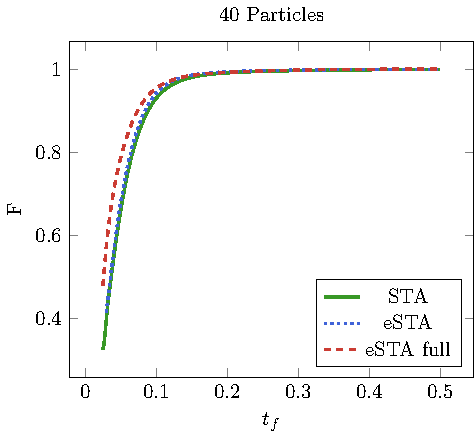
\includegraphics[width = \textwidth]{gfx/fidelity_compare_40.pdf}
	\caption{Comparison between the fidelity for 40 particles and for different final times, we can see eSTA outperforming the STA counterparts in both cases and it is more noticeable when eSTA is applied to the original version of the Bose Hubbard Hamiltonian.}
	\label{fig:FidelityCompare40}
\end{figure}
\begin{figure}[t]
	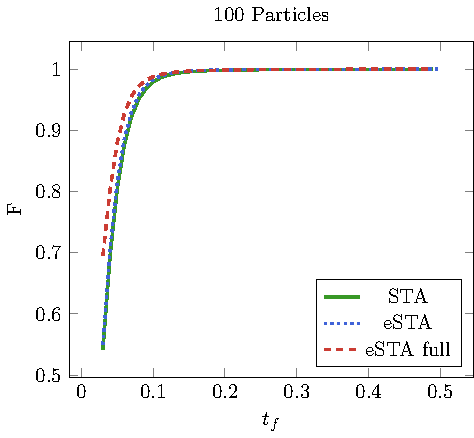
\includegraphics[width = \textwidth]{gfx/fidelity_compare_100.pdf}
	\caption{Similar comparison with 100 particles, again the figure shows the best performances obtained using eSTA. We can also see how the approximation is more stable for smaller final times when compared to the other figure with less particles.}
	\label{fig:FidelityCompare100}
\end{figure}

\bibliography{bibliography}
\end{document}
